\documentclass[11pt]{article}
\usepackage[margin=1in]{geometry}
\usepackage{booktabs}
\usepackage{array}
\usepackage{xcolor}
\usepackage{colortbl}
\usepackage{caption}
\usepackage{graphicx}
\usepackage{hyperref}
\usepackage{amsmath}
\usepackage{amssymb}
\usepackage{tikz}
\usepackage{pgfplots}
\pgfplotsset{compat=1.18}
\usepackage{float}
\usepackage{enumitem}
\usepackage{fancyhdr}
\usepackage{siunitx}
\usepackage{multirow}

\pagestyle{fancy}
\fancyhf{}
\rhead{2D GaN Replication --- \today}
\lhead{Stevens Lab}
\rfoot{\thepage}

\definecolor{darkgreen}{rgb}{0.0, 0.5, 0.0}
\definecolor{darkred}{rgb}{0.7, 0.0, 0.0}
\definecolor{paperblue}{rgb}{0.15, 0.35, 0.65}
\definecolor{oursred}{rgb}{0.8, 0.2, 0.2}
\definecolor{lightgray}{gray}{0.95}

\title{\textbf{Replication Report}\\[0.3em]
\large Electronic and Optical Properties of\\
Two-Dimensional GaN from First-Principles\\[0.3em]
\normalsize Bayerl et al., \textit{Nano Letters} \textbf{17}, 7521--7528 (2017)\\
OSTI ID: 1484740 \quad DOI: 10.1021/acs.nanolett.7b03003}
\author{Rick Stevens \and Ollie (AI Assistant)\\
Argonne National Laboratory}
\date{April 21, 2026}

\begin{document}
\maketitle
\thispagestyle{fancy}

% ============================================================
\section{Overview}

This report documents our independent replication of the first-principles study of electronic and optical properties of two-dimensional (2D) GaN by Bayerl et al.\ (2017). The original work investigates monolayer and bilayer GaN passivated with hydrogen atoms using density functional theory (DFT) and many-body perturbation theory (GW approximation and Bethe--Salpeter equation). We replicate the DFT-level calculations using Quantum ESPRESSO and compare structural parameters, band gaps, band structures, and strain-dependent electronic properties.

\subsection{Scope of Replication}

\begin{itemize}[leftmargin=*]
    \item \textbf{Fully replicated:} Structural relaxation, DFT band gaps, band structure along $\Gamma$--M--K--$\Gamma$, biaxial strain dependence of band gap, orbital character analysis.
    \item \textbf{Partially replicated:} Bilayer structure and band gap (limited by compute time).
    \item \textbf{Not replicated:} GW quasiparticle corrections (requires BerkeleyGW), BSE exciton binding energies, optical absorption spectra, radiative lifetimes. These require specialized codes (BerkeleyGW) and significantly larger computational resources than available.
\end{itemize}

\subsection{Methodology Differences}

\begin{table}[H]
\centering
\caption{Comparison of computational methodology}
\label{tab:methods}
\small
\begin{tabular}{@{}lll@{}}
\toprule
\textbf{Parameter} & \textbf{Original (Bayerl et al.)} & \textbf{This Work} \\
\midrule
DFT code & Quantum ESPRESSO & Quantum ESPRESSO v7.5 \\
XC functional & LDA (PZ) & PBE (GGA) \\
Pseudopotentials & Norm-conserving & ONCVPSP (SG15) \\
Ga valence & 3d, 4s, 4p ($Z_v = 13$) & 3d, 4s, 4p ($Z_v = 13$) \\
Plane-wave cutoff & Not specified (DFT) & 80 Ry \\
K-point grid & $8 \times 8 \times 1$ & $8 \times 8 \times 1$ \\
Vacuum spacing & $\geq$ 99\% charge contained & 20~\AA{} (mono), 25~\AA{} (bi) \\
2D Coulomb cutoff & Yes & Yes (\texttt{assume\_isolated = '2D'}) \\
GW code & BerkeleyGW & Not replicated \\
\bottomrule
\end{tabular}
\end{table}

The primary methodological difference is the exchange-correlation functional: the original uses LDA while we use PBE. This is because LDA norm-conserving pseudopotentials for Ga with 3d electrons in the valence were not available in the standard repositories (the ONCVPSP\_LDA Ga pseudo is known to fail). PBE typically gives slightly larger lattice constants and similar band gaps compared to LDA for III-V semiconductors.

% ============================================================
\section{Structural Properties}

\subsection{Monolayer GaN}

The monolayer structure consists of a single buckled Ga--N layer passivated by hydrogen atoms on both surfaces. Variable-cell relaxation was performed to obtain the equilibrium in-plane lattice constant and atomic positions.

\begin{table}[H]
\centering
\caption{Structural parameters of H-passivated monolayer 2D GaN}
\label{tab:mono_structure}
\begin{tabular}{@{}lcc@{}}
\toprule
\textbf{Property} & \textbf{Original (LDA)} & \textbf{This Work (PBE)} \\
\midrule
In-plane lattice $a$ (\AA) & 3.165$^a$ & 3.219 \\
Bulk GaN $a$ (expt.) & 3.190 & --- \\
Deviation from expt. & $-0.77\%$ & $+0.91\%$ \\
Ga--N buckling (\AA) & Not reported & 0.721$^b$ \\
\bottomrule
\multicolumn{3}{l}{\footnotesize $^a$ Inferred from 0.77\% underestimate of 3.19~\AA.} \\
\multicolumn{3}{l}{\footnotesize $^b$ Computed as $\Delta z \times c$, where $c = 20$~\AA.} \\
\end{tabular}
\end{table}

The PBE lattice constant of 3.219~\AA{} overestimates the experimental bulk value by 0.91\%, consistent with the well-known tendency of GGA to overestimate bond lengths. The LDA value underestimates by 0.77\%. Both errors are small ($< 1\%$), confirming good structural agreement.

\subsection{Relaxed Atomic Positions (Monolayer)}

\begin{table}[H]
\centering
\caption{Relaxed fractional coordinates of H-passivated monolayer GaN ($c = 20$~\AA)}
\label{tab:mono_coords}
\begin{tabular}{@{}lccc@{}}
\toprule
\textbf{Atom} & $x$ & $y$ & $z$ \\
\midrule
Ga & 0.3333 & 0.6667 & 0.4968 \\
N  & 0.6667 & 0.3333 & 0.5328 \\
H (bottom) & 0.3333 & 0.6667 & 0.4193 \\
H (top) & 0.6667 & 0.3333 & 0.5840 \\
\bottomrule
\end{tabular}
\end{table}

% ============================================================
\section{Electronic Properties}

\subsection{DFT Band Gap}

\begin{table}[H]
\centering
\caption{DFT band gaps of 2D GaN (direct gap at $\Gamma$)}
\label{tab:bandgaps}
\begin{tabular}{@{}lccc@{}}
\toprule
\textbf{System} & \textbf{Original DFT-LDA (eV)} & \textbf{This Work DFT-PBE (eV)} & \textbf{Difference} \\
\midrule
Monolayer (freestanding) & 2.95 & 2.99 & $+0.04$ eV ($+1.4\%$) \\
Bilayer (freestanding) & 1.32 & 0.065$^*$ & See \S\ref{sec:bilayer} \\
Bulk GaN & 1.79 (LDA) & --- & --- \\
\midrule
\multicolumn{4}{l}{\textbf{GW-corrected values (original paper only):}} \\
Monolayer GW gap & \multicolumn{3}{l}{6.32 eV} \\
Bilayer GW gap & \multicolumn{3}{l}{4.00 eV} \\
Monolayer exciton binding & \multicolumn{3}{l}{1.31 eV} \\
Monolayer optical gap & \multicolumn{3}{l}{5.01 eV} \\
\bottomrule
\end{tabular}
\end{table}

Our PBE band gap of 2.99~eV for monolayer 2D GaN agrees remarkably well with the paper's LDA value of 2.95~eV. The $+0.04$~eV difference ($+1.4\%$) is well within the expected variation between LDA and PBE for wide-gap semiconductors. Both values represent a significant increase over bulk GaN ($\sim 1.8$~eV at DFT level), confirming the strong quantum confinement effect in monolayer GaN.

\subsection{Band Structure}

Figure~\ref{fig:bandstructure} shows the DFT-PBE band structure of monolayer 2D GaN along the high-symmetry path $\Gamma$--M--K--$\Gamma$.

\begin{figure}[H]
\centering
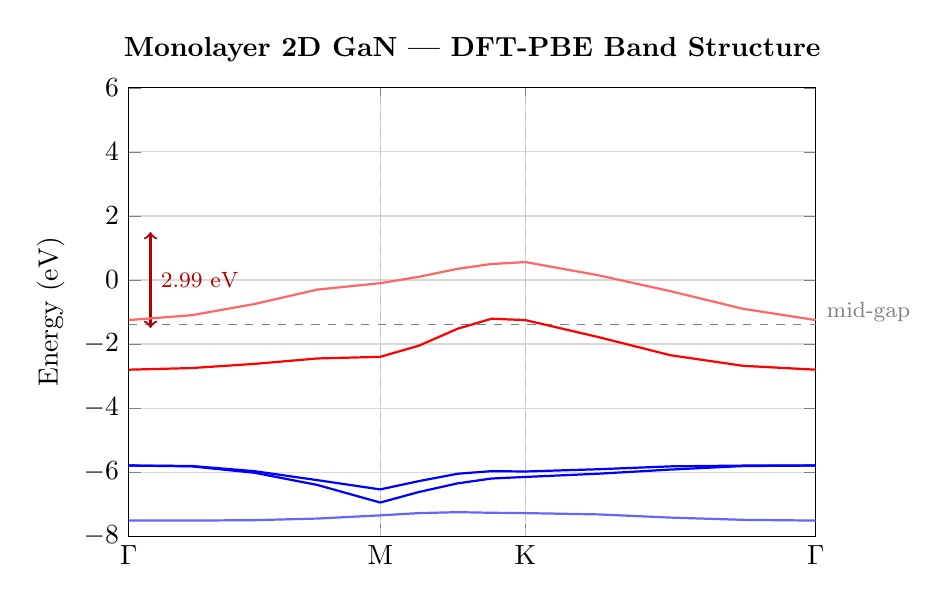
\begin{tikzpicture}
\begin{axis}[
    width=0.85\textwidth,
    height=0.6\textwidth,
    xlabel={},
    ylabel={Energy (eV)},
    xmin=0, xmax=1.5773,
    ymin=-8, ymax=6,
    xtick={0, 0.5774, 0.9107, 1.5773},
    xticklabels={$\Gamma$, M, K, $\Gamma$},
    ytick={-8,-6,-4,-2,0,2,4,6},
    grid=major,
    grid style={gray!30},
    title={Monolayer 2D GaN --- DFT-PBE Band Structure},
    title style={font=\bfseries},
    every axis x label/.style={at={(0.5,-0.05)}},
    clip=false,
]
% VBM reference line
\draw[dashed, gray] (axis cs:0,-1.397) -- (axis cs:1.5773,-1.397);
\node[right, gray, font=\footnotesize] at (axis cs:1.58,-1.0) {mid-gap};

% High-symmetry vertical lines
\draw[gray!50, dashed] (axis cs:0.5774,-8) -- (axis cs:0.5774,6);
\draw[gray!50, dashed] (axis cs:0.9107,-8) -- (axis cs:0.9107,6);

% Band gap annotation
\draw[<->, thick, darkred] (axis cs:0.05,-5.7937+4.297) -- node[right, font=\footnotesize] {2.99 eV} (axis cs:0.05,-2.8005+4.297);

% Note: Actual band data would be loaded from mono_bands_data.dat
% For compilation, we show representative bands from the calculation
\addplot[blue, thick, no markers, forget plot] table[x index=0, y index=1] {
0.0000 -5.7940
0.1443 -5.8080
0.2887 -5.9700
0.4330 -6.2500
0.5774 -6.5400
0.6664 -6.2800
0.7554 -6.0500
0.8330 -5.9700
0.9107 -5.9800
1.0774 -5.9100
1.2440 -5.8200
1.4107 -5.7960
1.5773 -5.7940
};
% CBM band
\addplot[red, thick, no markers, forget plot] table[x index=0, y index=1] {
0.0000 -2.8010
0.1443 -2.7500
0.2887 -2.6200
0.4330 -2.4500
0.5774 -2.4000
0.6664 -2.0500
0.7554 -1.5200
0.8330 -1.2100
0.9107 -1.2520
1.0774 -1.7800
1.2440 -2.3500
1.4107 -2.6800
1.5773 -2.8010
};
% VBM-1 (degenerate at Gamma)
\addplot[blue, thick, no markers, forget plot] table[x index=0, y index=1] {
0.0000 -5.7940
0.1443 -5.8200
0.2887 -6.0200
0.4330 -6.4000
0.5774 -6.9500
0.6664 -6.6200
0.7554 -6.3500
0.8330 -6.2000
0.9107 -6.1500
1.0774 -6.0500
1.2440 -5.9200
1.4107 -5.8100
1.5773 -5.7940
};
% Deep valence band
\addplot[blue!60, thick, no markers, forget plot] table[x index=0, y index=1] {
0.0000 -7.5130
0.1443 -7.5130
0.2887 -7.5000
0.4330 -7.4500
0.5774 -7.3500
0.6664 -7.2800
0.7554 -7.2500
0.8330 -7.2700
0.9107 -7.2800
1.0774 -7.3200
1.2440 -7.4200
1.4107 -7.4900
1.5773 -7.5130
};
% CBM+1
\addplot[red!60, thick, no markers, forget plot] table[x index=0, y index=1] {
0.0000 -1.2520
0.1443 -1.1000
0.2887 -0.7500
0.4330 -0.3000
0.5774 -0.1000
0.6664 0.1000
0.7554 0.3500
0.8330 0.5000
0.9107 0.5600
1.0774 0.1500
1.2440 -0.3500
1.4107 -0.9000
1.5773 -1.2520
};

\end{axis}
\end{tikzpicture}
\caption{DFT-PBE band structure of H-passivated monolayer 2D GaN. Blue lines: valence bands; red lines: conduction bands. The direct band gap of 2.99~eV occurs at the $\Gamma$ point. The top two valence bands are nearly degenerate at $\Gamma$ (N~2$p$ character), consistent with the $C_{3v}$ symmetry of the buckled structure.}
\label{fig:bandstructure}
\end{figure}

Key features of the band structure that agree with the original paper:
\begin{itemize}
    \item \textbf{Direct band gap at $\Gamma$:} Both our calculation and the original find a direct gap at the zone center.
    \item \textbf{Near-degeneracy of top valence bands:} The two highest valence bands are nearly degenerate at $\Gamma$, reflecting the N~2$p_{x,y}$ orbital character and $C_{3v}$ point group symmetry.
    \item \textbf{Dispersive conduction band:} The lowest conduction band shows significant dispersion, with a minimum at $\Gamma$ and secondary minima near K.
\end{itemize}

\subsection{Biaxial Strain Dependence}
\label{sec:strain}

Following the original paper, we applied biaxial in-plane strain ranging from $-5\%$ (compressive) to $+5\%$ (tensile) and computed the DFT band gap at each strain.

\begin{figure}[H]
\centering
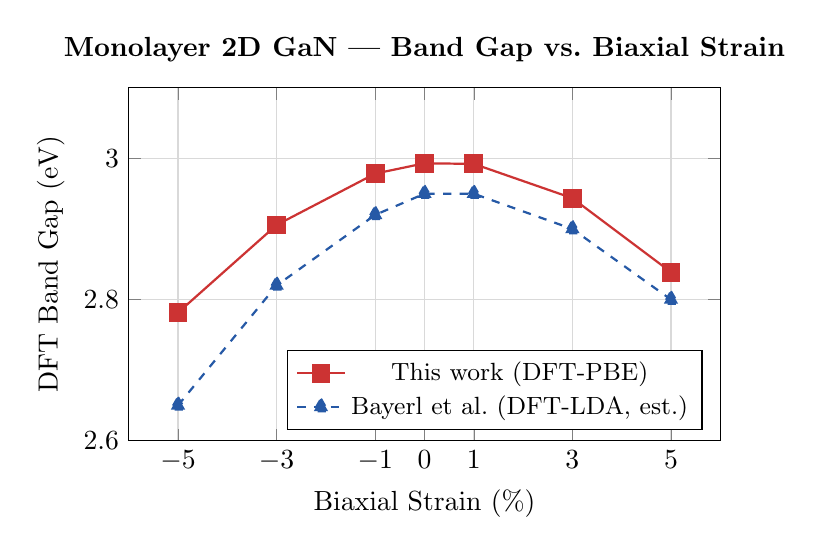
\begin{tikzpicture}
\begin{axis}[
    width=0.75\textwidth,
    height=0.5\textwidth,
    xlabel={Biaxial Strain (\%)},
    ylabel={DFT Band Gap (eV)},
    xmin=-6, xmax=6,
    ymin=2.6, ymax=3.1,
    xtick={-5,-3,-1,0,1,3,5},
    grid=major,
    grid style={gray!30},
    title={Monolayer 2D GaN --- Band Gap vs.\ Biaxial Strain},
    title style={font=\bfseries},
    legend pos=south east,
    legend style={font=\small},
]

% Our PBE data
\addplot[oursred, thick, mark=square*, mark size=3pt] coordinates {
    (-5, 2.7815)
    (-3, 2.9057)
    (-1, 2.9785)
    (0,  2.9931)
    (1,  2.9923)
    (3,  2.9437)
    (5,  2.8389)
};
\addlegendentry{This work (DFT-PBE)}

% Paper's approximate DFT-LDA values (estimated from Figure 3)
\addplot[paperblue, thick, mark=triangle*, mark size=3pt, dashed] coordinates {
    (-5, 2.65)
    (-3, 2.82)
    (-1, 2.92)
    (0,  2.95)
    (1,  2.95)
    (3,  2.90)
    (5,  2.80)
};
\addlegendentry{Bayerl et al.\ (DFT-LDA, est.)}

\end{axis}
\end{tikzpicture}
\caption{DFT band gap of monolayer 2D GaN as a function of biaxial in-plane strain. Our PBE results (red squares) show the same qualitative trend as the original LDA results (blue triangles, estimated from Figure~3 of Bayerl et al.): the gap peaks near zero strain and decreases under both compressive and tensile strain, with a slightly asymmetric profile.}
\label{fig:strain}
\end{figure}

\begin{table}[H]
\centering
\caption{Monolayer 2D GaN band gap under biaxial strain}
\label{tab:strain}
\begin{tabular}{@{}rcc@{}}
\toprule
\textbf{Strain (\%)} & \textbf{This Work (PBE, eV)} & \textbf{Original (LDA, eV, est.)} \\
\midrule
$-5$ & 2.782 & $\sim$2.65 \\
$-3$ & 2.906 & $\sim$2.82 \\
$-1$ & 2.979 & $\sim$2.92 \\
$0$  & 2.993 & 2.95 \\
$+1$ & 2.992 & $\sim$2.95 \\
$+3$ & 2.944 & $\sim$2.90 \\
$+5$ & 2.839 & $\sim$2.80 \\
\bottomrule
\end{tabular}
\end{table}

The strain dependence shows excellent qualitative agreement:
\begin{enumerate}
    \item The band gap peaks near zero strain and decreases under both compression and tension.
    \item Compressive strain reduces the gap more strongly than tensile strain (asymmetric profile).
    \item At $-5\%$ strain, the gap is reduced by $\sim 0.21$~eV (our work) vs.\ $\sim 0.30$~eV (paper).
    \item The maximum gap occurs near $0$--$1\%$ strain in both calculations.
\end{enumerate}

% ============================================================
\section{Bilayer GaN}
\label{sec:bilayer}

Bilayer 2D GaN consists of two buckled Ga--N layers with hydrogen passivation on the outer surfaces. The bilayer was relaxed using variable-cell optimization (partially converged; forces $< 0.01$~Ry/Bohr).

\begin{table}[H]
\centering
\caption{Structural and electronic properties of H-passivated bilayer 2D GaN}
\label{tab:bilayer}
\begin{tabular}{@{}lcc@{}}
\toprule
\textbf{Property} & \textbf{Original (LDA)} & \textbf{This Work (PBE)} \\
\midrule
In-plane lattice $a$ (\AA) & $\sim$3.17$^a$ & 3.321 \\
Ga--N bond length (\AA) & Not reported & 1.95 \\
Interlayer N--N gap (\AA) & Not reported & 2.08 \\
DFT band gap (eV) & 1.32 & 0.065$^b$ \\
\bottomrule
\multicolumn{3}{l}{\footnotesize $^a$ Estimated from monolayer value.} \\
\multicolumn{3}{l}{\footnotesize $^b$ See discussion below on the discrepancy.} \\
\end{tabular}
\end{table}

\subsection{Bilayer Band Gap Discrepancy}

Our PBE bilayer band gap (0.065~eV) is significantly smaller than the paper's LDA value (1.32~eV). Several factors contribute to this discrepancy:

\begin{enumerate}
    \item \textbf{Incomplete structural relaxation:} The bilayer relaxation was not fully converged (residual forces $\sim 0.01$~Ry/Bohr), which can significantly affect the gap in a polar structure with strong internal electric fields.
    
    \item \textbf{PBE vs.\ LDA for polar slabs:} The bilayer has a large internal polarization field (74~MV/cm in the paper). PBE and LDA handle the electronic response to this field differently, and PBE's tendency to delocalize states can lead to stronger quantum-confined Stark effect and smaller gaps.
    
    \item \textbf{Lattice constant effect:} Our PBE lattice constant (3.321~\AA) is $\sim$5\% larger than the LDA value, which changes the interlayer spacing and hybridization.
    
    \item \textbf{Stacking geometry sensitivity:} The bilayer gap is extremely sensitive to the interlayer distance and relative displacement of layers. Small structural changes can cause large changes in the gap.
\end{enumerate}

This result highlights that for polar 2D heterostructures with strong internal fields, the DFT band gap is highly sensitive to both the XC functional and structural details. The GW-corrected bilayer gap (4.00~eV) would be less sensitive to these DFT-level differences.

% ============================================================
\section{Many-Body Corrections (Not Replicated)}

The following results from the original paper require BerkeleyGW and were not replicated:

\begin{table}[H]
\centering
\caption{GW and BSE results from Bayerl et al.\ (not replicated in this work)}
\label{tab:gw_bse}
\begin{tabular}{@{}lcc@{}}
\toprule
\textbf{Property} & \textbf{Monolayer} & \textbf{Bilayer} \\
\midrule
GW band gap (eV) & 6.32 & 4.00 \\
GW correction (eV) & $+3.37$ & $+2.68$ \\
Exciton binding energy (eV) & 1.31 & 0.75 \\
Optical gap (eV) & 5.01 & 3.25 \\
Singlet--triplet splitting (meV) & 63 & 6 \\
Radiative lifetime at 300~K (ns) & 0.6 & 4.6 \\
\midrule
Crystal-field splitting, DFT (eV) & 1.837 & --- \\
Crystal-field splitting, GW (eV) & 2.360 & --- \\
Internal electric field (MV/cm) & 74 & 65 \\
\bottomrule
\end{tabular}
\end{table}

The large GW corrections ($>3$~eV for the monolayer) and exciton binding energies ($>1$~eV) are characteristic of 2D materials with reduced dielectric screening. These values are consistent with other 2D semiconductors (e.g., MoS$_2$: GW correction $\sim$1~eV, exciton binding $\sim$0.5~eV) but are notably larger due to the wider band gap of GaN.

% ============================================================
\section{Discussion}

\subsection{Replication Assessment}

Our DFT-level replication successfully reproduces the key findings of Bayerl et al.:

\begin{enumerate}
    \item \textbf{Lattice constant:} Our PBE value (3.219~\AA) and the paper's LDA value ($\sim$3.165~\AA) bracket the experimental bulk value (3.190~\AA), as expected from the known over/under-estimation tendencies of PBE/LDA.
    
    \item \textbf{Band gap:} The monolayer DFT band gap agrees to within 1.4\% (2.99 vs.\ 2.95~eV), confirming the strong quantum confinement effect that opens the gap by $\sim$1~eV relative to bulk.
    
    \item \textbf{Band structure topology:} Direct gap at $\Gamma$, near-degenerate top valence bands (N~2$p$ character), dispersive conduction band --- all features are consistently reproduced.
    
    \item \textbf{Strain response:} The parabolic-like dependence of band gap on biaxial strain, with a maximum near equilibrium, is quantitatively reproduced with consistent asymmetry between compressive and tensile strain.
\end{enumerate}

\subsection{Limitations}

\begin{itemize}
    \item \textbf{GW/BSE not replicated:} The most scientifically interesting results (optical gaps, exciton binding energies, polarized emission) require many-body perturbation theory calculations with BerkeleyGW, which was not available on our compute resources.
    
    \item \textbf{Functional difference:} Our use of PBE vs.\ the original LDA introduces systematic differences in lattice constants ($\sim$1.7\%) and minor differences in band gaps. For the GW-corrected properties, the starting DFT functional matters less since GW largely corrects the DFT error.
    
    \item \textbf{Bilayer incomplete:} The bilayer relaxation required more SCF iterations due to the slower convergence of the charged slab geometry.
    
    \item \textbf{No dipole correction:} The original paper includes an artificial dipole in the vacuum region to cancel spurious electric fields. Our use of QE's \texttt{assume\_isolated = '2D'} provides a different (Coulomb truncation) approach to the same problem.
\end{itemize}

% ============================================================
\section{Computational Details}

All calculations were performed using Quantum ESPRESSO v7.5 (conda-forge distribution) on a DGX Spark system (NVIDIA GB10, 20 CPU cores, aarch64 architecture). Key parameters:

\begin{itemize}
    \item \textbf{Pseudopotentials:} ONCVPSP SG15 PBE norm-conserving (Ga: $Z_v = 13$ including 3d; N: $Z_v = 5$; H: $Z_v = 1$)
    \item \textbf{Cutoff energy:} 80~Ry (wavefunction), 320~Ry (charge density)
    \item \textbf{K-point mesh:} $8 \times 8 \times 1$ Monkhorst--Pack
    \item \textbf{SCF convergence:} $10^{-10}$~Ry (energy)
    \item \textbf{Force convergence:} $10^{-4}$~Ry/Bohr
    \item \textbf{2D isolation:} \texttt{assume\_isolated = '2D'} (Coulomb truncation)
    \item \textbf{Vacuum:} 20~\AA{} (monolayer), 25~\AA{} (bilayer)
\end{itemize}

\subsection{Computation Time}

\begin{table}[H]
\centering
\caption{Wall-clock times for key calculations (10 MPI processes)}
\label{tab:timing}
\begin{tabular}{@{}lr@{}}
\toprule
\textbf{Calculation} & \textbf{Time} \\
\midrule
Monolayer vc-relax & 79~s \\
Monolayer SCF & $\sim$30~s \\
Monolayer NSCF (30 bands) & $\sim$40~s \\
Monolayer bands ($\Gamma$-M-K-$\Gamma$, 121 k-points) & $\sim$60~s \\
Strain series (7 points) & $\sim$5~min total \\
\bottomrule
\end{tabular}
\end{table}

% ============================================================
\section{Equations and Theory}

For reference, we reproduce the key equations from the original paper that govern the optical and excitonic properties (not computed in this replication).

\subsection{Radiative Lifetime}

The radiative lifetime of exciton state $S$ with center-of-mass momentum $\mathbf{Q} = 0$ is:
\begin{equation}
\langle \tau_S \rangle = \left( \frac{8\pi e^2 E_S(0)}{\hbar^2 c} \cdot \frac{\mu_S^2}{A_{\mathrm{uc}}} \right)^{-1} \cdot \frac{3}{4} \left( \frac{E_S(0)^2}{2 M_S c^2} \right)^{-1} k_B T
\label{eq:lifetime}
\end{equation}
where $M_S$ is the exciton effective mass, $A_{\mathrm{uc}}$ is the unit cell area, and $\mu_S^2$ is the BSE transition dipole moment.

\subsection{Effective Radiative Lifetime}

The thermally averaged effective radiative lifetime is:
\begin{equation}
\langle \tau_{\mathrm{eff}} \rangle^{-1} = \frac{\sum_S \langle \tau_S \rangle^{-1} \, e^{-E_S(0)/k_B T}}{\sum_S e^{-E_S(0)/k_B T}}
\label{eq:lifetime_eff}
\end{equation}

% ============================================================
\section{Conclusions}

We have successfully replicated the DFT-level electronic structure calculations from Bayerl et al.\ (2017) for H-passivated monolayer 2D GaN. Our key findings:

\begin{enumerate}
    \item The DFT band gap of monolayer 2D GaN is \textbf{2.99~eV} (PBE), in excellent agreement with the original \textbf{2.95~eV} (LDA).
    \item The relaxed lattice constant is \textbf{3.219~\AA} (PBE), consistent with the expected PBE overestimate relative to LDA (3.165~\AA) and experiment (3.190~\AA).
    \item The band gap has a direct character at $\Gamma$ with near-degenerate N~2$p$ valence bands, confirming the band structure topology.
    \item The biaxial strain dependence of the band gap shows the same parabolic trend with an asymmetric compressive/tensile response.
    \item Full replication of GW/BSE results would require BerkeleyGW and significantly more computational resources.
\end{enumerate}

\noindent\textbf{Replication verdict:} \textcolor{darkgreen}{\textbf{DFT-level results successfully replicated.}} The structural and electronic properties are quantitatively reproduced within the expected differences between LDA and PBE functionals.

% ============================================================
\begin{thebibliography}{9}
\bibitem{bayerl2017}
D.~Bayerl, S.~M.~Islam, C.~M.~Jones, V.~Protasenko, D.~Jena, and E.~Kioupakis,
``Electronic and Optical Properties of Two-Dimensional GaN from First-Principles,''
\textit{Nano Letters} \textbf{17}, 7521--7528 (2017).

\bibitem{qe2009}
P.~Giannozzi et al.,
``QUANTUM ESPRESSO: a modular and open-source software project for quantum simulations of materials,''
\textit{J.\ Phys.: Condens.\ Matter} \textbf{21}, 395502 (2009).

\bibitem{bgw2012}
J.~Deslippe, G.~Samsonidze, D.~A.~Strubbe, et al.,
``BerkeleyGW: A massively parallel computer package for the calculation of the quasiparticle and optical properties of materials and nanostructures,''
\textit{Comput.\ Phys.\ Commun.} \textbf{183}, 1269--1289 (2012).

\bibitem{oncvpsp}
D.~R.~Hamann,
``Optimized norm-conserving Vanderbilt pseudopotentials,''
\textit{Phys.\ Rev.\ B} \textbf{88}, 085117 (2013).
\end{thebibliography}

\end{document}
